\documentclass{article}
\usepackage{tikz}
\begin{document}
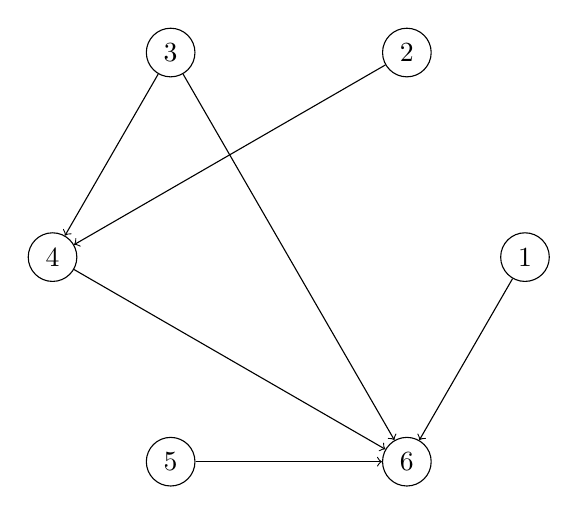
\begin{tikzpicture}[->,node distance=2cm]
\tikzstyle{every node}=[circle,draw]
\node (1) at (3.0,0.0) {1};
\node (2) at (1.5000000000000004,2.598076211353316) {2};
\node (3) at (-1.4999999999999993,2.598076211353316) {3};
\node (4) at (-3.0,3.6739403974420594e-16) {4};
\node (5) at (-1.5000000000000013,-2.598076211353315) {5};
\node (6) at (1.5000000000000004,-2.598076211353316) {6};
\draw[->] (1) -- (6);
\draw[->] (2) -- (4);
\draw[->] (3) -- (6);
\draw[->] (3) -- (4);
\draw[->] (4) -- (6);
\draw[->] (5) -- (6);
\end{tikzpicture}
\end{document}
